\renewcommand\thechapter{\Roman{chapter}}
\chapter{MÉTODO} \label{ch:metodo} \thispagestyle{fancy}
\renewcommand\thechapter{\arabic{chapter}}
%%%%%%%%%%%%%%%%%%%%%%%%%%%%%%%%%%%%%%%%%%%%%%%%%%%%%%%%%%%%%%%%%%%%%%%%%%%%
En este capitulo se abordará la explicación de los pasos que se deben llevar a cabo para finalizar el simulador, los pasos serán mostrados por un diagrama de flujo a continuación de una breve explicación de cada bloque finalizando con el material que se va a requerir para poder terminar todos los pasos.\\

\section{Sujeto}
\begin{itemize}
\item Investigadores del área de arquitectura de computadoras con enfoque en aceleradores implementados a nivel de hardware.
\end{itemize}

\section{Procedimiento}

\begin{figure}[!h]
\centering
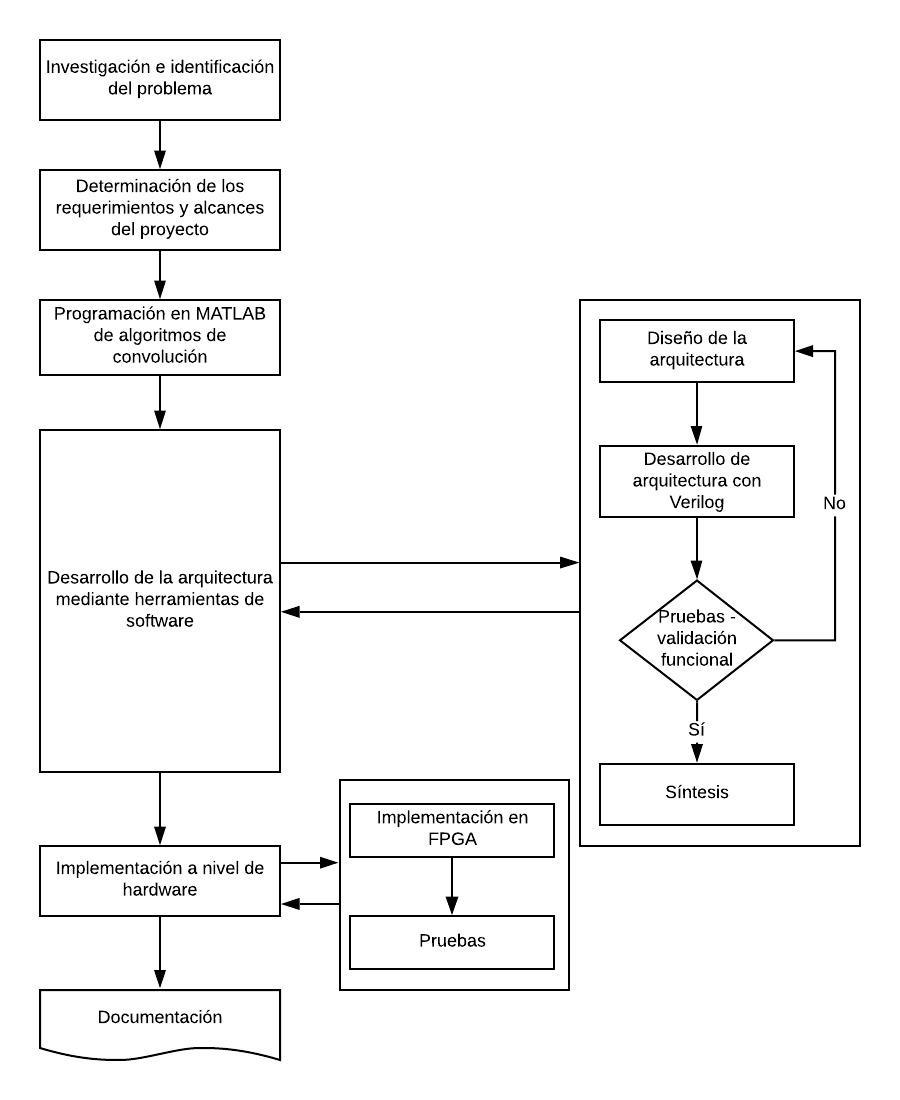
\includegraphics[width=0.6\textwidth, height=0.6\textheight]{./figs/procedimiento}\\
\caption{Diagrama de flujo}
\label{diagramaflujo}
\end{figure}

\newpage
Como se puede ver en la figura \ref{diagramaflujo} se muestran los pasos a seguir para poder desarrollar dicho proyecto, se dará inicio revisando artículos los cuales sean del mismo tema, desde que año se ha dado inicio a la creación de herramientas para aplicar el concepto de la enseñanza para el aprendizaje, continuando base a lo anterior se mostrarán los alcances que tiene la investigación hasta donde se planea llegar, dicho lo anterior se dará inicio al desarrollo creando el diseño de un brazo robótico en SolidWorks a continuación éste se tendrá que modificar para poder abrirlo en MatLab el cual es un programa dentro de simulink con el que ayuda a interactuar de manera virtual con objetos llamado V realm builder, ya que el robot tenga todos los parámetros se usará JMathLink para poder que haya una interacción entre MatLab y Java3D, con esto se logrará que la animación tenga mayor fluidez.

\section{Materiales y Herramientas}
\begin{itemize}
\item Laptop Dell Inspiron 13-5378
\item Mathworks Matlab R2015a
\item Xilinx ISE 14.7
\color{red}
\item agregar los que faltan (FPGA, OS(?))
\end{itemize}
